\documentclass[a4paper]{jacow}

\usepackage{mathtools}
\usepackage{amsmath}
\usepackage{xfrac}
\usepackage{xparse}
\usepackage{subcaption}
\usepackage{graphicx}
\usepackage{url}
\usepackage{paralist}

\let\oldvec\vec
\renewcommand{\vec}{\boldsymbol}
\DeclareDocumentCommand{\bkt}{sm}{\IfBooleanTF{#1}{\left[ #2 \right]}{\left(#2\right)}}
\DeclareDocumentCommand{\ddt}{m}{\frac{\mathrm{d} {#1}}{\mathrm{d} t}}
\DeclareDocumentCommand{\pddx}{mO{t}O{}}{\frac{\partial^{#3} {#1}}{\partial {#2}^{#3}}}
\newcommand{\w}{\omega}
\newcommand{\W}{\Omega}
\newcommand{\avg}[1]{\langle {#1} \rangle}
\newcommand{\Traj}{\mathcal T}
\DeclareDocumentCommand{\Stab}{s}{\mathcal{S}\IfBooleanT{#1}{\vert_{\W_y=0}}}
\newcommand{\Fail}{\mathcal F}
\newcommand{\D}{\mathcal D}
\DeclareDocumentCommand{\g}{s}{\gamma\IfBooleanT{#1}{_{eff}}}
\newcommand{\CO}{\mathrm{CO}}
\newcommand{\nbar}{\bar n}

\begin{document}
\title{SIMULATION OF THE GUIDE FIELD FLIPPING PROCEDURE FOR THE FREQUENCY DOMAIN METHOD}
\author{A. E. Aksentyev\textsuperscript{1,2,3}\thanks{alexaksentyev@gmail.com},
  Y. V. Senichev\textsuperscript{3} \\
  \textsuperscript{1} National Research Nuclear University ``MEPhI,'' Moscow, Russia \\
  \textsuperscript{2} Institut f\"ur Kernphysik, Forschungszentrum J\"ulich, J\"ulich, Germany\\
  \textsuperscript{3} Institute for Nuclear Research of the Russian Academy of Sciences, Moscow, Russia}
\maketitle

\begin{abstract}
  The spin vector of a particle injected into a perfectly aligned storage ring precesses about
  the vertically-orientated guide field. In the presence of an Electric Dipole Moment (EDM),
  the spin precession axis acquires a proportional radial component.
  However, in an imperfect ring, rotational magnet misalignments induce a radial component
  to the spin precession axis, related to the Magnetic Dipole Moment (MDM). In the Frequency Domain Method,
  this additional precession is dealt with by consecutively injecting the beam in opposite directions,
  and constructing the EDM estimator as the sum of the clockwise and counter-clockwise
  vertical plane precession frequencies. Since the radial MDM component changes sign
  when the magnetic field direction is reversed, it cancels in the sum, leaving only the EDM effect. 
  In order to reproduce the guide field magnitude with a precision sufficient for
  the cancellation of the MDM effect, we propose to calibrate the guide field via
  the horizontal plane precession frequency. In the present work we describe the algorithm of
  the field flipping procedure, and do a numerical simulation.
\end{abstract}

\section{Spin dynamics in a storage ring}
The dynamics of a spin-vector $\vec s$ in a magnetic field $\vec B$ and an electrostatic field $\vec E$
is described by the Thomas-BMT equation. Its generalized version, accounting for the effect of
the particle's electric dipole moment, can be written in the rest frame as:
\begin{subequations}
  \begin{align}
    \ddt{\vec s} &= \vec s\times \bkt{\vec\W_{MDM} +\vec\W_{EDM}}, \label{eq:TBMT_main}
    \intertext{where the magnetic (MDM) and electric (EDM) dipole moment angular velocities
      $\vec\W_{MDM}$ and $\vec\W_{EDM}$ }
    \vec\W_{MDM} &= \frac qm \bkt*{G\vec B - \bkt{G - \frac{1}{\gamma^2-1}}\frac{\vec E\times\vec\beta}{c}},\label{eq:TBMT_MDM} \\
    \vec\W_{EDM} &= \frac qm \frac\eta2 \bkt*{\frac{\vec E}c + \vec\beta\times \vec B}.\label{eq:TBMT_EDM}
  \end{align}
\end{subequations}
In the above equations, $m,~q,~G=(g-2)/2$ are, respectively, the mass, charge, and anomalous magnetic moment
of the particle; $\beta = \sfrac{v_0}{c}$ is its normalized speed; $\gamma$ its Lorentz-factor.
The EDM factor $\eta$ is defined by the equation $d = \eta\frac{q}{2mc}$, in which $d$ is the particle EDM,
$s$ its spin.

\section{BNL Frozen Spin method}
The original method for the measurement of the electric dipole moment of an elementary particle
was first proposed by the Storage Ring EDM Collaboration~\cite{BNL:SREDM} of Brookhaven National Laboratory.
In the proposed method,~\cite{BNL:Deuteron2008} a longitudinally-polarized beam is injected into a storage ring
designed on the basis of the Frozen Spin (FS) concept: by applying a radial electric field
$E_r = \frac{GB_yc\beta\gamma^2}{1-G\beta^2\gamma^2}$,~\cite[p.~10]{BNL:Deuteron2008} the MDM component
in~\eqref{eq:TBMT_main} is set to zero: $\vec\W_{MDM} = \vec 0$. Then, any tilting of
the beam polarization vector out of the horizontal plane is attributed to the presence of an EDM;
specifically, the vertical component $P_y$ grows as
\[
P_y =  P\frac{\W_{edm}}{\W}\sin\bkt{\W t + \Theta_0} \approx P\W_{EDM}\cdot t,
\]
where $\W = \sqrt{\W_{EDM}^2 + \W_{MDM}^2}$.~\cite[p.~8]{BNL:Deuteron2008}

This method has two inherent weaknesses, due to the smallness of the hypothesized EDM value:
\begin{inparaenum}[\itshape a\upshape)]
\item the expected polarization tilt angle after 1,000 seconds is on the order of
  microradians,~\cite[p.~18]{BNL:Deuteron2008}
  which makes for difficult polarimetry~\cite[p.~6]{Mane:SpinWheel} and
\item the main systematic effect, $\W_{syst} \approx \frac{\mu\avg{E_y}}{c\beta\gamma^2}$
  ($\mu$ being the MDM of the particle)~\cite[p.~10]{BNL:Deuteron2008} must be reduced to less than
  $\W_{EDM}$ if one is to measure the polarization tilt angle.
\end{inparaenum}
The systematic error is caused by accelerator element alignment error. For a practical value of
100$\mu$m of element installation uncertainty, this means a $\W_{syst}$ on the order of
50 rad/sec.~\cite{Senichev:FDM}

Both these problems can be mitigated if the net spin precession frequency is used as the EDM observable.

\section{Frequency Domain Method}
The Frequency Domain Methodology (FDM)~\cite{Senichev:FDM} was designed specifically to address the problem
of element alignment uncertainty. The FS condition condition is fulfilled as in the BNL method; however,
instead of the polarization tilt angle, the combined MDM+EDM precession frequency is measured in two cases:
once when the beam is injected clockwise, and once counter-clockwise. The EDM-effect is extracted by
comparing the measured frequencies. When the guide field polarity is reversed $\vec B \mapsto -\vec B$,
$\vec\beta \mapsto -\vec\beta$, and $\vec E \mapsto \vec E$, precession frequency components change thus:
\begin{subequations}
  \begin{align}
    \W_x^{CW/CCW} &= \W_x^{MDM, CW/CCW} + \W_x^{EDM, CW/CCW}, \notag\\
    \W_x^{MDM, CW} &= -\W_x^{MDM, CCW} \equiv \W_x^{MDM},  \notag\\
    \W_x^{EDM, CW} &= \W_x^{EDM, CCW} \equiv \W_x^{EDM}, \label{eq:CW_CCW_MDM}
    \intertext{and the EDM estimator}
    \hat\W_x^{EDM} &:= \frac12\bkt{\W_x^{CW} + \W_x^{CCW}} \label{eq:FDM_estimator} \\
    &= \W_x^{EDM} + \underbrace{\frac12\bkt{\W_x^{MDM, CW} + \W_x^{MDM, CCW}}}_{\varepsilon \to 0}.
  \end{align}
\end{subequations}

In order to guarantee that $\varepsilon$ is less than the required EDM measurement precision, i.e. that
equation~\eqref{eq:CW_CCW_MDM} holds with sufficient accuracy,
a guide field flipping algorithm has been devised, that uses the horizontal plane precession frequency
as a means to calibrating the guide field. 

\section{Calibration algorithm}
The goal of flipping the direction of the guide field is to accurately reproduce the radial component
of the MDM spin precession frequency due to element misalignment.

Let $\Traj$ denote the set of all trajectories that a particle might follow in the accelerator.
$\Traj = \Stab \bigcup \Fail$, where $\Stab$ is the set of all stable trajectories, $\Fail$ are all trajectories
such that if a particle gets on one, it will be lost from the bunch.

Calibration is done in two phases:
\begin{enumerate}
\item In the first phase, the guide field value is set so that the beam particles are injected onto trajectories
  $t\in\Stab$.
\item In the second phase, it is fine-tuned further, so as to fulfill the FS condition in the horizontal plane:
  by doing this, we select the subset $\Stab*\subset\Stab$ of trajectories for which $\W_y = 0$.
\end{enumerate}

Spin tune (and hence precession frequency) is an injective function of the
effective Lorentz-factor $\g*$~\cite{Aksentev:DecohIPAC19}, which means
$\W_y(\g*^1) = \W_y(\g*^2) \rightarrow \g*^1 = \g*^2$. The trajectory space $\Traj$ is partitioned into equivalence
classes according to the value of $\g*$: trajectories characterized by the same $\g*$ are equivalent
in terms of their spin dynamics (possess the same spin tune and invariant spin axis direction),
and hence belong to the same equivalence class.
Since $\W_y(\g*)$ is injective, there exists a unique $\g*^0$ at which $\W_y(\g*^0)=0$:
\[
[\W_y=0] = [\g*^0] \equiv \Stab*.
\]

If the lattice didn't use sextupole fields for the suppression of decoherence,
$\Stab*$ would be a singleton set. We have shown in~\cite{Aksentev:DecohIPAC19} that if sextupoles are
utilized, then $\exists\D\subset\Stab$ such that $\forall t_1,t_2\in\D$:
$\nu_s(t_1) = \nu_s(t_2)$, $\nbar(t_1) = \nbar(t_2)$. By adjusting the guide field strength we equate
$\D=\Stab*$, and hence $\Stab*$ contains multiple trajectories.~\footnote{Strictly speaking,
  even if sextupoles are used there remains some negligible dependence of spin tune
  on the particle orbit length (linear decoherence effects, cf.~\cite{Aksentev:DecohIPAC19}).
  Because of that, the equalities for spin tune and $\nbar$ are approximate, and the set $\Stab*$
  should be viewed as fuzzy:
  we will consider trajectories for which $|\W_y|<\delta$ for some small $\delta$ as belonging to $[\W_y=0]$.}

Therefore, once we ensured that the beam polarization does not precess in the horizontal plane,
all of the beam particles have $\g*^0$, equal for the CW and CCW beams.

\section{Simulation}
In order to confirm that the proposed calibration procedure works, we need to show that:
\begin{enumerate}
\item $\Stab*^{CW} = \Stab*^{CCW}$, that is $\W_y=0$ for the same set of trajectories (equivalently,
  the same $\g*$) in the CW and CCW cases.
\item $\forall t_1,t_2\in\Stab*^{CCW}$: $\nu_s(t_1) = \nu_s(t_2)$, $\nbar(t_1) = \nbar(t_2)$, i.e., the same
  sextupole fields reduce decohrerence in the CW and CCW beams.
\end{enumerate}

We do this by first computing the function $\nu_s(z)$ (where $z$ is the particle's horizontal, vertical, or
momentum offset from the reference particle) for the CW and CCW beams; and then compute their discrepancy
$\epsilon(z) = \nu_s^{CW}(z) - \nu_s^{CCW}(z)$. If the discrepancy is small in a wide range of $z$, then
\begin{enumerate}
\item sextupole decoherence suppression works for both beams without gradient value change;
\item spin tune (respectively $\g*$) is equal for both beams, and hence their Spin Wheels roll at the
  same rate.
\end{enumerate}

In the simulation, we use an imperfect FS lattice~\cite{Senichev:Lattices}, in which the E+B
spin rotator elements are tilted about the optic axis by angles $\alpha\sim N(0, 5\cdot 10^{-4})$ radians.
The simulation is repeated three times; each time only one sextupole family is turned on.

The beam's kinetic energy is 270.00 MeV. We compute third-order Taylor expansions of the
spin and orbital transfer maps.

The main body of the simulation consists in the following: using the TSS~\cite[p.~41]{COSYINF:BeamPhysMan}
procedure
of COSY Infinity we compute the $\nu_s$ and $\nbar$ third-order Taylor expansions for the lattice traversed
in the forward direction.
Then, using the combinations of procedures MR and SMR~\cite[p.~233]{Eremey:Thesis}, we reverse
the lattice's orbital and spin transfer maps, and compute $\nu_s$ and $\nbar$
for the reversed lattice (as it is seen by the counter-circulating beam).

\section{Results}

\begin{figure}[h]
  \centering
  \begin{subfigure}{\linewidth}\centering
    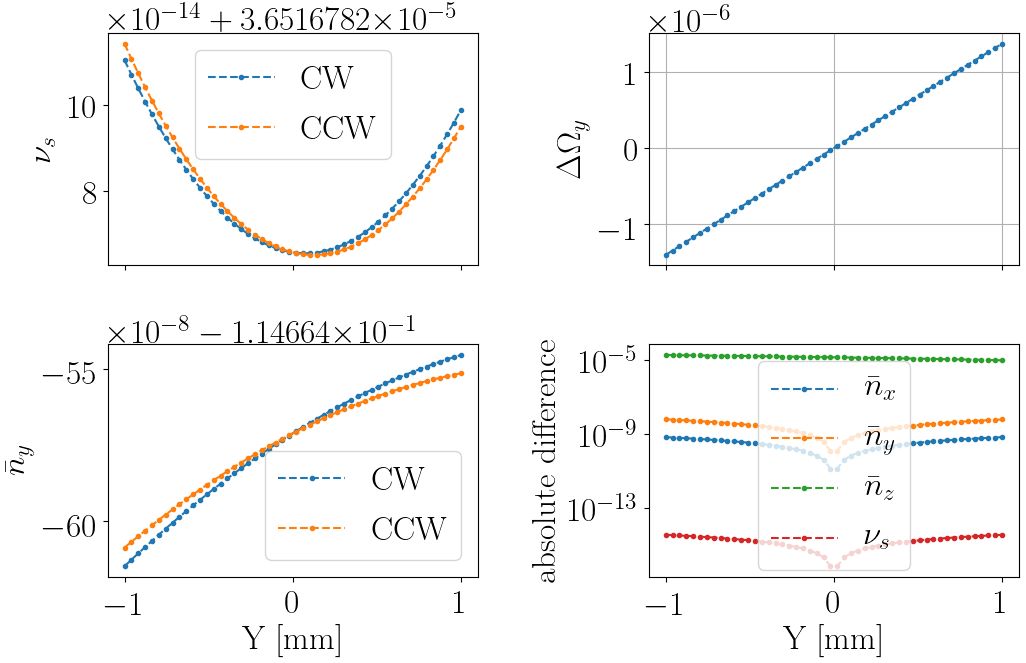
\includegraphics[width=\linewidth]{../img/IPAC19/GFF_stune_range_Y}
    \caption{Spin tune and invariant spin axis dependencies on the particle vertical offset
      from the reference orbit\label{fig:Y:calib_plot:stune}}
  \end{subfigure}
  \begin{subfigure}{\linewidth}\centering
    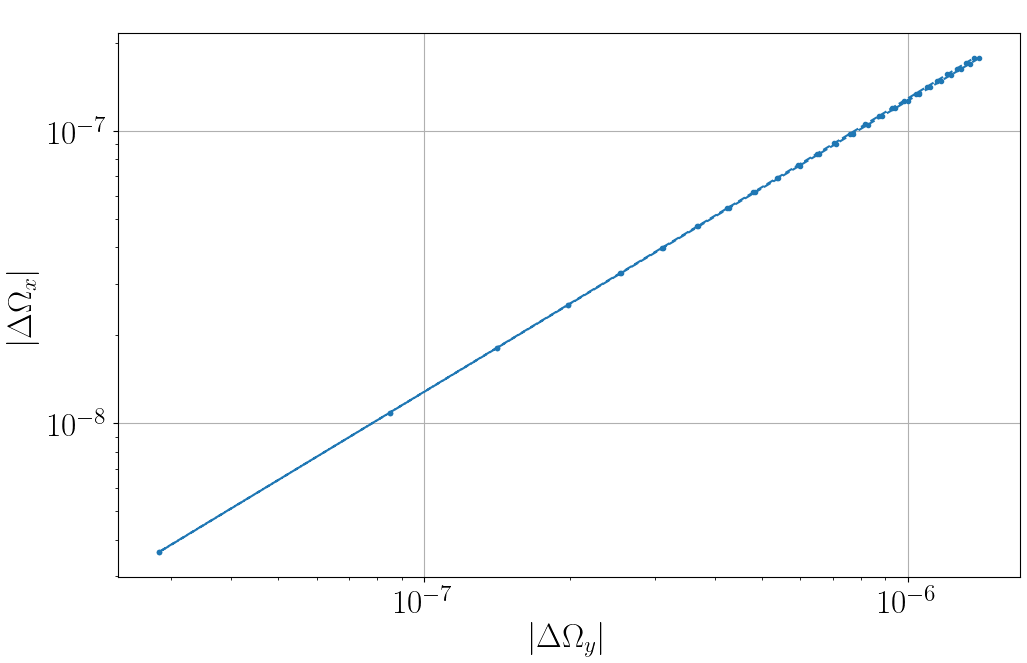
\includegraphics[width=\linewidth]{../img/IPAC19/GFF_omegas_range_Y}
    \caption{Difference between the CW and CCW radial plane precession frequencies
      vs the corresponding horizontal plane frequencies (calibration plot)\label{fig:Y:calib_plot:omegas}}
  \end{subfigure}
  \caption{Simulation results for the decoherence caused by
    vertical plane betatron motion\label{fig:Y:calib_plot}}
\end{figure}

In Figure~\ref{fig:Y:calib_plot} are shown the $\nu_s$ and $\nbar_y$ dependencies on the particle's
vertical offset from the reference orbit, when the corresponding sextupoles are operational. Specifically, in
Figure~\ref{fig:Y:calib_plot:stune} one can observe that there's a difference between the CW and CCW beams
in the values of spin tune and invariant spin axis vertical component for trajectories
deviating from the reference orbit. Figure~\ref{fig:Y:calib_plot:omegas} indicates that if one can make the
difference between the CW and CCW particle's horizontal plane precession frequencies
smaller than $10^{-7}$ rad/sec,
the difference between their vertical plane precession frequencies will be smaller than $10^{-8}$ rad/sec.
This confirmes that the equalization of the vertical plane MDM precession frequencies of counter-circulating
beams by means of equalizing their horizontal plane precession frequencies is a viable technique.

\begin{figure}[h]
  \centering
  \begin{subfigure}{\linewidth}
    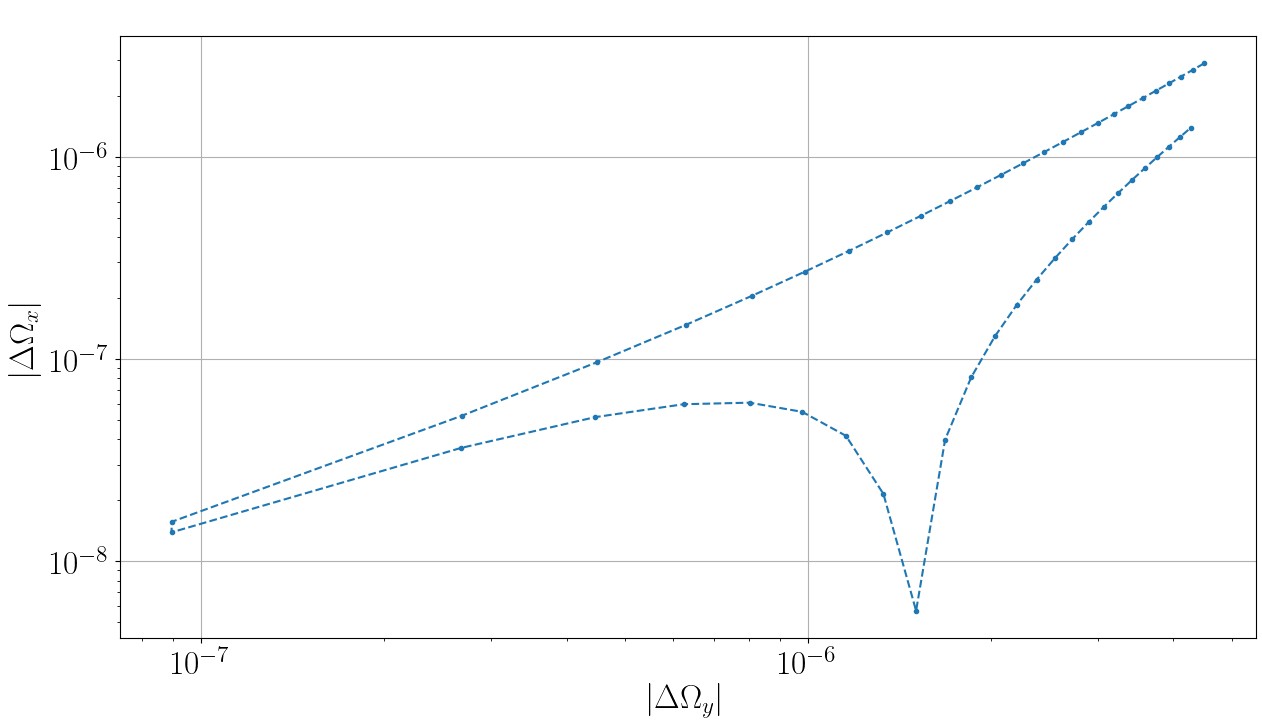
\includegraphics[width=\linewidth]{../img/IPAC19/GFF_omegas_range_X}
    \caption{Horizontal betatron motion case\label{fig:X:calib_plot:omegas}}
  \end{subfigure}
  \begin{subfigure}{\linewidth}
    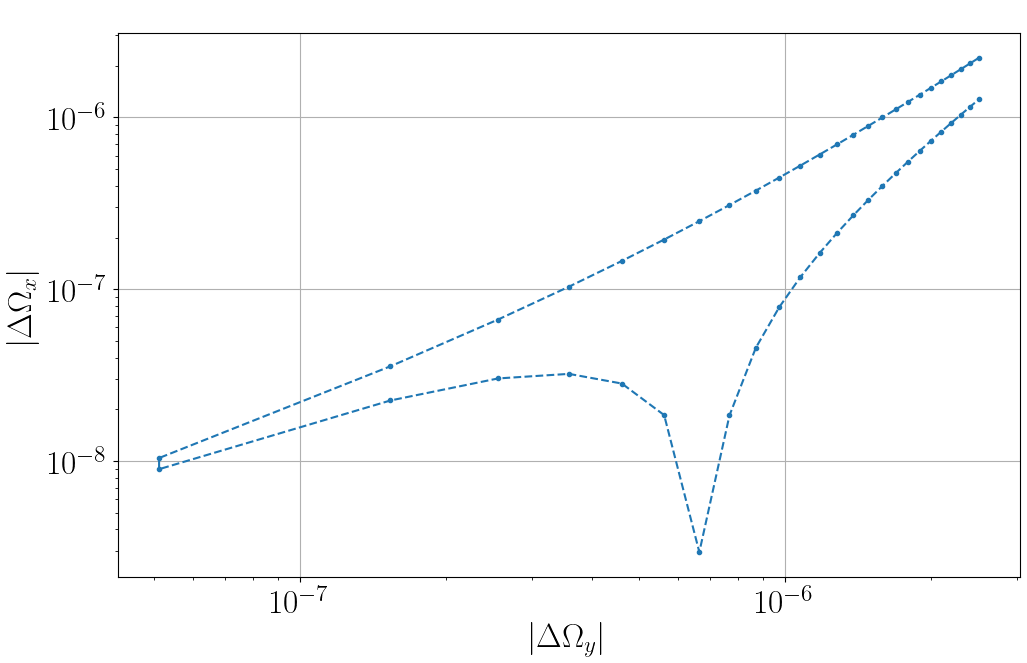
\includegraphics[width=\linewidth]{../img/IPAC19/GFF_omegas_range_D}
    \caption{Synchrotron motion case\label{fig:D:calib_plot:omegas}}
  \end{subfigure}
  \caption{Calibration plots in the cases of decoherence caused by horizontal betatron motion
    and synchtorton oscillations\label{fig:calib_plot:omegas}}
\end{figure}

In Figure~\ref{fig:calib_plot:omegas} you see the calibration plots when we varied the horizontal 
offset, and the momentum offset.

\begin{thebibliography}{9}

\bibitem{BNL:SREDM}
  M. Bai et al., SREDM Collaboration website: \url{https://www.bnl.gov/edm/}.

\bibitem{BNL:Deuteron2008}
  D. Anastassopoulos et at., (srEDM Collaboration), ``Search for a permanent electric dipole moment of
  the deuteron nucleus at the $10^{-29}~e\cdot cm$ level,'' proposal as submitted to the BNL PAC, April 2008.

\bibitem{Mane:SpinWheel}
  S. Mane, ``A distillation of Koop's idea of the Spin Wheel,'' arXiv:1509.01167 [physics]
  \url{http://arxiv.org/abs/1509.01167}.
  
\bibitem{Senichev:FDM}
  Y. Senichev, A. Aksentev, A. Ivanov, E. Valetov, ``Frequency domain method of the search for
  the deuteron electric dipole moment in a storage ring with imperfections,'' arxiv:1711.06512 [physics.acc-ph]
  \url{https://arxiv.org/abs/1711.06512}.

\bibitem{COSY:SpinTuneMapping}
  A. Saleev et al., (JEDI Collaboration), ``Spin tune mapping as a novel tool to probe
  the spin dynamics in storage rings.'' Phys. Rev. Accel. Beams 20 (2017) no.7, 072801.

\bibitem{Aksentev:DecohIPAC19}
  A. Aksentev, Y. Senichev, ``Spin decoherence in the Frequency Domain Method for the search of a particle EDM,''
  presented at the 10th International Particle Accelerator Conf. (IPAC’19), Melbourne, Australia,
  May. 2019, paper 2738, this conference.

\bibitem{Senichev:Lattices}
  Y. Senichev, S. Andrianov, S. Chekmenev, M. Berz, E.Valetov. ``Investigation of Lattice for Deuteron EDM Ring,''
  Proc. of ICAP15 (2015). \url{http://accelconf.web.cern.ch/AccelConf/ICAP2015/papers/modbc4.pdf}.

\bibitem{COSYINF:BeamPhysMan}
  M. Berz, K. Makino. COSY INFINITY 10.0 Beam Physics Manual.

\bibitem{Eremey:Thesis}
  E. Valetov, ``Field modeling, symplectic tracking, and spin decoherence for the EDM and muon g-2 lattices.''
  PhD tehsis, Michigan State University, Michigan, USA.
  \url{http://collaborations.fz-juelich.de/ikp/jedi/public_files/theses/valetovphd.pdf}

%% \bibitem{Senichev:IPAC13}
%%   Y. Senichev, R. Maier, D. Zyuzin, N. Kulabukhova, (JEDI Collaboration), ``Spin tune decoherence effects in electro- and magnetostatic structures.'' Proc. of IPAC13 (2013).

%% \bibitem{COSY:Website}
%%   M. Berz, Kyoko Makino, COSY Infinity website: \url{cosyinfinity.org}


  
\end{thebibliography}
\end{document}
